\chapter{Configuring Networks with NETCONF}

In this chapter, we explore the practical implementation of NETCONF (Network Configuration Protocol) for configuring networks in a Cisco router. Building upon the foundational understanding of DHCP, NAT, SSH, and the fundamentals of NETCONF established earlier, we delve into the specifics of leveraging NETCONF to streamline network configuration processes.

Before delving further, it is crucial to first explore the fundamental base operations of NETCONF. Understanding these operations provides a solid foundation for effectively leveraging NETCONF in network configuration management.

\section{NETCONF base operations}

The NETCONF protocol supports a set of low-level operations for retrieving and managing device configuration information.As detailed before, the operations are specified through XML elements. NETCONF also supports additional operations based on each device's capabilities:

\begin{itemize}
    \item \texttt{<get>} : Retrieves all or part of the information about the running configuration and device state.
    \item \texttt{<get-config>}: Retrieves all or part of the configuration information available from a specified configuration datastore.
    \item \texttt{<edit-config>}: Submits all or part of a configuration to a target configuration datastore.
    \item \texttt{<copy-config>}: Creates or replaces a target configuration datastore with the information from another configuration datastore.
    \item \texttt{<delete-config>}: Deletes a target configuration datastore, but only if it is not running.
    \item \texttt{<lock>}: Locks a target configuration datastore, unless a lock already exists on any part of that datastore.
    \item \texttt{<unlock>}: Releases a lock on a configuration datastore that was previously locked through a \texttt{<lock>} operation.
    \item \texttt{<close-session>}: Requests the NETCONF server to gracefully terminate an open session.
    \item \texttt{<kill-session>}: Forces a session's termination, causing current operations to be aborted.
\end{itemize}

\section{Python code structure}

There are multiple ways to configure networks using NETCONF. Some common approaches include using command-line interfaces (CLI) on network devices, network management tools with built-in NETCONF support, or developing custom automation scripts. Python is a preferred choice for configuring networks with NETCONF due to its ease of use, rich ecosystem, comprehensive documentation, and most importantly, its integration capabilities.

\subsection{Libraries}

The ncclient library is a popular Python implementation used for interacting with NETCONF-enabled devices. It provides a high-level API (Application Programming Interface) that simplifies the process of establishing NETCONF sessions, retrieving device information, and configuring network devices. Its key benefits include:

\begin{enumerate}
    \item Simplified NETCONF Communication:
    \begin{itemize}
      \item Abstracts low-level details of the NETCONF protocol, providing an intuitive interface for developers.
      \item Allows developers to focus on automation logic without the need to delve into protocol intricacies.
    \end{itemize}
    
    \item Easy Connection Establishment:
    \begin{itemize}
      \item Handles authentication mechanisms (e.g., SSH) for establishing secure NETCONF sessions.
      \item Provides a seamless channel for communication with NETCONF-enabled devices.
    \end{itemize}
    
    \item Configuration Management:
    \begin{itemize}
      \item Facilitates retrieval and manipulation of device configuration using NETCONF.
      \item Simplifies the retrieval of configuration data, application of configuration changes, and validation of resulting configurations.
    \end{itemize}
    
    \item Error Handling and Validation:
    \begin{itemize}
      \item Includes built-in mechanisms for error handling and structured error responses.
      \item Enables developers to validate configuration changes and effectively handle exceptions.
    \end{itemize}

\end{enumerate}

\subsection{Session establishment}

In this section, we discuss the process of establishing a NETCONF session using the manager.connect() method as an example. This method is part of the ncclient library and allows us to establish a secure connection with the router.

\begin{lstlisting}[style=pythonStyle, caption={Session establishment.}, backgroundcolor=\color{codebackground}]
                    with manager.connect(
                          host="192.168.1.1",
                          port=830,
                          username="admin", 
                          password="nabil",
                          hostkey_verify=False
                          ) as m:           
\end{lstlisting}


\begin{enumerate}
    \item \texttt{manager.connect()}: The \texttt{manager.connect()} method initiates the process of establishing a NETCONF session.
    \item \texttt{host}: This parameter specifies the IP address of the router (in this case, $192.168.1.1$).
    \item \texttt{port}: The \texttt{port} parameter defines the port number used for the NETCONF communication, which is typically set to 830.
    \item \texttt{username} and \texttt{password}: These parameters provide the necessary authentication credentials to access the router.
    \item \texttt{hostkey\_verify}: By setting this parameter to \texttt{False}, host key verification for the SSH connection is disabled. This option can be useful during testing or when connecting to devices with self-signed or invalid SSH certificates. However, exercise caution and ensure the security implications are understood before using this option.
    \item \texttt{with} statement: The \texttt{with} statement ensures that the NETCONF session is properly established and automatically closed when the block of code inside the \texttt{with} statement finishes execution.
\end{enumerate}
\subsection{Filter}
The filter is a mechanism used to retrieve specific subsets of configuration or operational data from a network device. It allows us to define criteria for selecting the desired data elements using XPath expressions. By utilizing the filter parameter in NETCONF operations, such as \texttt{<get-config>} or \texttt{<get>}, we can retrieve only the relevant information needed for our application or task. This targeted data retrieval capability enhances network management and automation by minimizing unnecessary data transfer, optimizing response times, and reducing network bandwidth usage. 

For example, for the \texttt{<get-config>} operation in NETCONF with Python, we can use the \textit{filter} parameter to retrieve only the interface configurations from a network device. By specifying a filter criterion using XPath expressions that target the interface elements, such as \texttt{`/interfaces/interface'}, we can narrow down the retrieved data to only the relevant interface information.

\begin{lstlisting}[style=pythonStyle, caption={Filter for interfaces.}, backgroundcolor=\color{codebackground}]
  netconf_filter = """
      <filter>
        <interfaces xmlns="urn:ietf:params:xml:ns:yang:ietf-interfaces">
          <interface></interface>
        </interfaces>
      </filter>"""          
\end{lstlisting}

\subsection{Configuration modification/retrieval and commit}

This section showcases the process of connecting to the router, making modifications to the configuration, retrieving the configuration, and committing the changes.

The following example focuses on modifying a router's configuration, specifically changing its interface configuration, and then committing the changes:
\begin{lstlisting}[style=pythonStyle, caption={Changing the interface.}, backgroundcolor=\color{codebackground}]
              with manager.connect(**device, hostkey_verify=False) as m:
                    # Lock the candidate datastore
                    m.lock('candidate')

                    # Edit the configuration in the candidate datastore
                    m.edit_config(target='candidate', config=filter)

                    # Validate the candidate configuration
                    m.validate()

                    # Commit the candidate configuration to apply the changes
                    m.commit()

                    # Unlock the candidate datastore
                    m.unlock('candidate')
              print("Interface changed successfully.")          
\end{lstlisting}

\begin{enumerate}
  \item Establishing a connection using the \texttt{manager.connect()} method.
  \item Locking the candidate configuration datastore to prevent concurrent modifications.
  \item Editing the configuration in the candidate datastore using the \texttt{edit\_config()} method.
  \item Validating the candidate configuration using the \texttt{validate()} method to ensure correctness.
  \item Committing the modified candidate configuration using the \texttt{commit()} method to apply the changes.
  \item Unlocking the candidate configuration datastore.
\end{enumerate}

\subsubsection{Limitation of Using Running Configuration Directly in Cisco CSR1000v}

When working with network devices, it is common to have the ability to directly modify the running configuration. However, it is important to note that not all devices support this feature. One such example is the Cisco CSR1000v router.

The Cisco CSR1000v router does not allow direct modifications to the running configuration. This limitation is revealed by examining the capabilities of the router through the use of NETCONF. The capabilities provided by the router specify the supported operations and features. In the case of the Cisco CSR1000v, the capabilities indicate that editing the running configuration directly is not available.

\begin{lstlisting}[style=pythonStyle, caption={Router CSR1000v capabilities.}, backgroundcolor=\color{codebackground}]
              urn:ietf:params:netconf:base:1.0
              urn:ietf:params:netconf:base:1.1
              urn:ietf:params:netconf:capability:candidate:1.0
              urn:ietf:params:netconf:capability:xpath:1.0
              urn:ietf:params:netconf:capability:validate:1.0
\end{lstlisting}

This limitation in modifying the running configuration directly with the Cisco CSR1000v router reinforces the importance of using a candidate configuration when making changes (Chapter\ref{chap:impl} provides the process of enabling the candidate datastore). By employing a candidate configuration, network administrators can safely apply and validate changes before committing them to the running configuration. This approach ensures greater control and reduces the risk of disrupting the network due to erroneous or incomplete configurations.

Understanding the limitations of the Cisco CSR1000v router in supporting direct modifications to the running configuration enables network administrators to adopt appropriate configuration management practices. By utilizing candidate configurations and committing changes only after thorough testing and validation, network stability and reliability can be maintained effectively.

\section{Python automation}
\subsection{Scenario}

In the context of a large institution such as a university, the establishment and management of a network infrastructure are critical for seamless communication and efficient resource allocation. One common scenario is the implementation of a centralized IP address pool shared by multiple routers within the network. This approach allows for optimal utilization of available IP addresses while accommodating the diverse needs of various departments, faculties, or network segments.

To ensure effective allocation of sub-networks within this shared IP pool, a systematic approach is required. By analyzing the specific requirements of each sub-network, such as the number of IP addresses needed for its operations, it becomes possible to devise an allocation strategy that fulfills the requirements. This approach allows for efficient utilization of IP resources, prevents IP address conflicts, and simplifies network management.

In this section, we will focus on the automation and, leveraging tools like the Python script provided in this report, the  allocation process can be streamlined. We will create a script that enables network administrators to input the desired number of IP addresses for each sub-network, and based on this information, it calculates the appropriate range of addresses and assigns them accordingly. The generated sub-networks can be further configured with relevant network parameters such as masks, DHCP server networks, and default routers.

The proposed solution offers a practical and efficient method for managing a large-scale network infrastructure within an institution. It provides the flexibility to allocate IP addresses based on individual sub-network requirements, ensuring optimized utilization of IP addresses while maintaining a coherent and manageable network architecture. This approach promotes scalability, adaptability, and ease of network administration, making it well-suited for complex environments like universities and other large institutions.

\subsection{Solving the Subnet Allocation Challenge}

\begin{itemize}
    \item[1.] \textbf{Router IP Address Requirement Assessment:} The first step is to assess the IP address requirements for each router. By understanding the number of IP addresses needed for their operations, we can allocate appropriate sub-networks. This information can be gathered through consultation with network administrators, department representatives, or through network traffic analysis.
    \item[2.] \textbf{Developing an Automated Subnet Allocation Script:}
    
    \begin{itemize}
        \item[a.] \textbf{Reordering the List of IP Requirements}

        To streamline the sub-network allocation process, it is beneficial to reorder the list of IP requirements in descending order. This reordering ensures that routers with larger IP address needs are given priority during the allocation process. By prioritizing routers with greater IP requirements, we can allocate larger sub-networks to accommodate their needs while maximizing the utilization of available IP addresses.

        \item[b.] \textbf{Visualizing the IP Pool as a Circular Space}

        To conceptualize the allocation process, we can envision the IP pool as a circular space, imagining a circle representing the entire pool of available IP addresses. Each router's IP requirement corresponds to a slice or segment within this circular space. The size of each slice is directly proportional to the number of IP addresses required by the router. By visualizing the IP pool in this manner, we can better understand the allocation process and optimize the sub-network assignments.


        \item[c.] \textbf{Allocating Subnets based on Slice Proportions}

        With the IP requirements reordered and the IP pool visualized as a circular space, the next step is to allocate sub-networks based on the proportions determined by each router's IP requirement. Starting from the router with the largest IP requirement, we assign a sub-network slice to that router that corresponds to its proportional share of the circular space. We then move on to the router with the second-highest IP requirement and allocate the next slice accordingly. This process continues until all routers have been assigned sub-networks.

        \item[d.] \textbf{Ensuring Efficient Resource Utilization}

        By following this systematic approach, we ensure that routers with larger IP requirements are allocated larger sub-networks, while routers with smaller IP requirements receive proportionally smaller sub-networks. This allocation strategy maximizes the utilization of available IP addresses, reduces IP address wastage, and avoids unnecessary sub-network fragmentation.
        
        \end{itemize}
\begin{figure}[h]
  \centering
  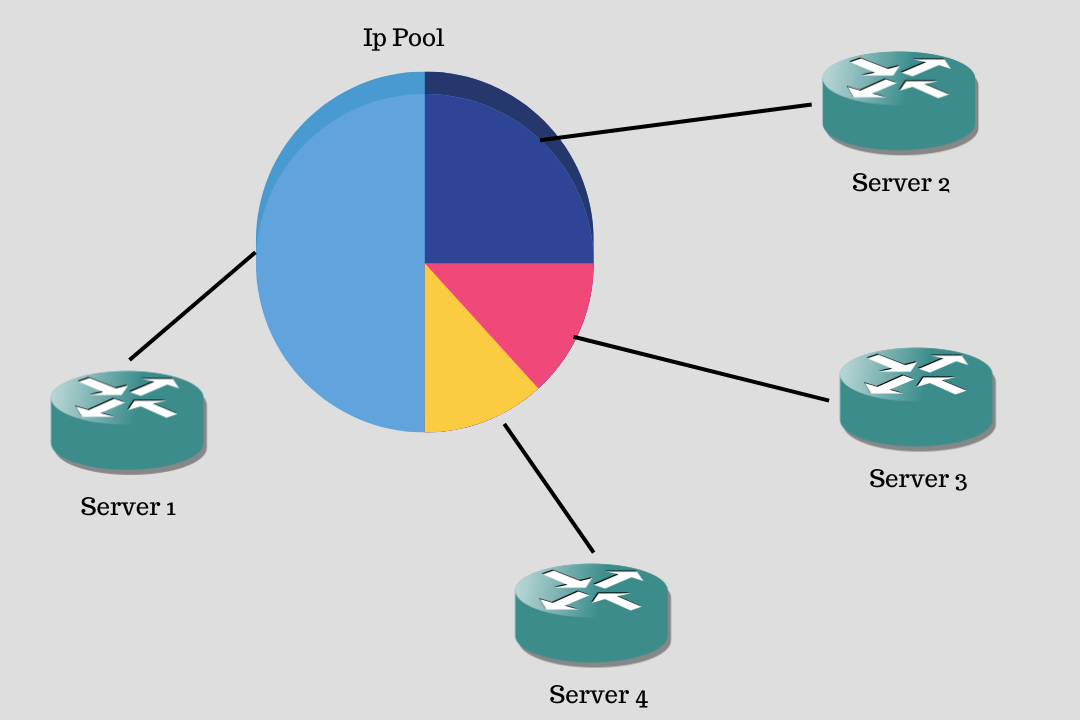
\includegraphics[width=0.5\linewidth]{Images/Pool.png}
  \caption{Visualizing the IP Pool as a Circular Space.}
\end{figure}

    \item[3.] \textbf{IP Pool Management:} It is essential to maintain an accurate inventory of the IP pool and track the allocation of sub-networks to ensure efficient resource utilization. Network administrators can use IP address management (IPAM) tools or custom scripts to monitor and manage the IP pool effectively.

    \item[4.] \textbf{Addressing IP Conflicts:} With multiple routers sharing a single IP pool, the risk of IP conflicts increases. Implementing mechanisms like DHCP servers and DHCP reservations can help mitigate IP conflicts and ensure proper IP address assignment within each sub-network.

    \item[5.] \textbf{Configuration and Documentation:} After the sub-network allocation process, configuring each router with the assigned sub-network, subnet masks, default routers, and other relevant network parameters is essential. Additionally, maintaining proper documentation, including address allocation records and network diagrams, aids in network troubleshooting and future expansion.
\end{itemize}


\subsection{Example: Router IP Address Requirement Assessment and Subnet Allocation}

To illustrate the process of router IP address requirement assessment and address allocation, let's consider a scenario with four routers in a large institution network. Each router has a specific number of IP addresses required for its operations, and we have a general subnet available for allocation.

\subsubsection{Router Information:}
\begin{itemize}
  \item Router A: Requires 80 IP addresses.
  \item Router B: Requires 40 IP addresses.
  \item Router C: Requires 50 IP addresses.
  \item Router D: Requires 150 IP addresses.
\end{itemize}

\subsubsection{General Subnet:}

The available general subnet is $192.168.0.0/23$, providing a total of 512 IP addresses.

\subsubsection{Router IP Address Requirement Assessment:}

To begin, we reorder the list of IP requirements in descending order:
\begin{itemize}
  \item Router D: 150 IP addresses
  \item Router A: 80 IP addresses
  \item Router B: 50 IP addresses
  \item Router C: 40 IP addresses
\end{itemize}


\subsubsection{Visualizing the IP Pool:}

We conceptualize the IP pool as a circular space, representing the available $192.168.0.0/23$ subnet. Each router's IP requirement corresponds to a slice or segment within this circular space. The size of each slice is directly proportional to the number of IP addresses required by the router.

\subsubsection{Allocating Subnets based on Slice Proportions:}

Starting with Router D, which has the highest IP requirement, we allocate a sub-network slice that fulfills its need for 150 IP addresses. Router A receives a subnet mask /24, which provides up to 256 addresses. It is worth noting that smaller sub-networks are not possible, since mask /25 only provides 128 addresses, so that the requirement of 150 addresses is not satisfied. Then a DHCP Server is configured correspondingly: 192.168.0.0  (192.168.0.0 - 192.168.0.255).
%
At this point there is another /24 sub-network available (or 2 /25, or 4 /26, etc.) to share among the rest of routers. Next, we move on to Router A, allocating a mask /25, and a DHCP Server Network: 192.168.0.0  (192.192.0.0 - 192.168.0.127). Again, we need to use the mask /25 to satisfy the requirement of addresses, since the sub-networks with mask /26 only provide 64 addresses.
%
For Router B, a sub-networks with a subnet mask /26 is granted, satisfying its need for 50 IP addresses. Finally, Router C is given another sub-network with  mask of /26 to accommodate its requirement of 40 IP addresses. Eventually, the whole pool of IP addresses is used.

\subsubsection{Testing Subnet Allocation Code}
The following listings showcase the input and outputs of the implemented management solution when used for the example described above.

\subsubsection{Input:}

\begin{lstlisting}[style=pythonStyle, caption={Routers informations input.}, backgroundcolor=\color{codebackground}]
              Enter the network and subnet in CIDR notation 
              (e.g., 10.10.0.0/23): 192.168.0.0/23
              Enter the number of routers: 4
              Enter the num_ips_router for Device1: 80
              Enter the num_ips_router for Device2: 50
              Enter the num_ips_router for Device3: 40
              Enter the num_ips_router for Device4: 150
\end{lstlisting}
\subsubsection{Output:}

\begin{lstlisting}[style=pythonStyle, caption={Output.}, backgroundcolor=\color{codebackground}]
              Device4
                Interface IP: 192.168.0.1
                Subnet Mask: 255.255.255.0 ( 24 )       
                DHCP Server Network: 192.168.0.0        
                DHCP Server Default Router: 192.168.0.1
              Device1
                Interface IP: 192.168.0.1
                Subnet Mask: 255.255.255.128 ( 25 )     
                DHCP Server Network: 192.168.0.0        
                DHCP Server Default Router: 192.168.0.1 

              Device2
                Interface IP: 192.168.0.1
                Subnet Mask: 255.255.255.192 ( 26 )     
                DHCP Server Network: 192.168.0.0        
                DHCP Server Default Router: 192.168.0.1 

              Device3
                Interface IP: 192.168.0.65
                Subnet Mask: 255.255.255.192 ( 26 )     
                DHCP Server Network: 192.168.0.64       
                DHCP Server Default Router: 192.168.0.65

\end{lstlisting}